\documentclass[conference]{IEEEtran}
\IEEEoverridecommandlockouts
\usepackage{cite}
\usepackage{amsmath,amssymb,amsfonts}
\usepackage{graphicx}
\usepackage{textcomp}
\usepackage{xcolor}
\usepackage{booktabs}
\usepackage{hyperref}
\usepackage{enumitem}
\setlist{noitemsep, topsep=1pt, parsep=0pt, partopsep=0pt}
\setlength{\abovecaptionskip}{2pt}
\setlength{\belowcaptionskip}{-5pt}

\def\BibTeX{{\rm B\kern-.05em{\sc i\kern-.025em b}\kern-.08em
    T\kern-.1667em\lower.7ex\hbox{E}\kern-.125emX}}
\begin{document}

\title{RoadFury: Transformer-Based Test Prioritization\\for Simulation-Based Testing of Self-Driving Cars}
\author{\IEEEauthorblockN{Author Name}
\IEEEauthorblockA{\textit{Dept.\ of Computer Science} \\
\textit{University Name}, City, Country \\
author@email.com}}
\maketitle

\begin{abstract}
When a self-driving car drifts off the road in simulation, the road's geometry-its sharp turns, S-curves, and spirals-is almost always the root cause. Yet existing test prioritization tools reduce this rich sequential structure to just three aggregate statistics, discarding the very ordering that makes a road dangerous. We present \textbf{RoadFury}, which preserves the full geometric sequence: a 10-channel feature matrix encoding curvature, heading, jerk, and positional context at every road point, processed by a Pre-LN Transformer Encoder trained with Stochastic Weight Averaging (SWA). After a systematic exploration of four paradigms-zero-shot LLMs, graph neural networks, visual CNNs, and sequential Transformers-we find that only the sequential approach consistently outperforms random ordering. Deployed as a gRPC service for the ICST~2026 SDC Testing Competition~\cite{b8}, RoadFury achieves APFD~=~\textbf{0.804\,$\pm$\,0.012}, establishing a new state of the art.
\end{abstract}

\begin{IEEEkeywords}
test prioritization, self-driving cars, Transformer, stochastic weight averaging, road geometry
\end{IEEEkeywords}

%=====================================================================
\section{Introduction}

Testing self-driving cars in high-fidelity simulators like BeamNG.tech is essential but expensive~\cite{b1,b2}: a single test can take tens of seconds to minutes, and suites easily grow to tens of thousands. As AI-driven navigation grows increasingly sophisticated~\cite{b16}, the demand for thorough simulation coverage only intensifies. \emph{Test prioritization} tackles this bottleneck by reordering tests so that failure-revealing cases run first, measured by the Average Percentage of Fault Detection (APFD)~\cite{b4}:
\vspace{-3pt}
\begin{equation}
\text{APFD}(\pi) = 1 - \frac{\sum_{i=1}^{m} TF_i}{n \cdot m} + \frac{1}{2n}
\end{equation}
where $n$ is total tests, $m$ failing tests, and $TF_i$ the rank of the $i$-th fault. A score of 1.0 means all failures are found first; 0.5 corresponds to random ordering.

Existing tools such as SDC-Scissor~\cite{b1,b2} and ITEP4SDC compute three aggregate statistics per road-mean segment length, angle change, and curvature-and feed them into a feedforward network. This approach collapses the road into a single point in feature space, discarding the \emph{sequential structure} that makes a road dangerous: the precise ordering of gentle straights followed by sudden hairpins.

A natural question arises: \emph{what is the right representation for road geometry?} We systematically explored four paradigms-zero-shot language models, graph neural networks, visual CNNs, and sequential Transformer encoding-and found that only the last consistently surpasses random ordering by a meaningful margin. This insight led to \textbf{RoadFury}: a 10-channel geometric feature representation processed by a Pre-LN Transformer Encoder~\cite{b11} with Stochastic Weight Averaging (SWA)~\cite{b6}. Prior work supports our design choices: systematic comparisons confirm Transformers outperform classical classifiers on sequential inputs~\cite{b15}; early-stage ML can predict AI-artifact outcomes from structural features~\cite{b14}; and SWA finds flatter optima that generalize better~\cite{b6}. Yoo and Harman~\cite{b4} provide a comprehensive survey of regression testing.

%=====================================================================
\section{Approach}

\subsection{Road Normalization and Feature Extraction}

Each test case is a variable-length sequence of 2D road control points. We resample all sequences to $L{=}197$ points via linear interpolation and extract 10 intrinsic geometric channels (Table~\ref{tab:features}), yielding a $(197{\times}10)$ translation- and rotation-invariant feature matrix, z-normalized with training-set statistics.

\begin{table}[t]
\caption{10-Channel Road Geometry Features}
\begin{center}
\setlength{\tabcolsep}{3pt}
{\small\begin{tabular}{cll}
\toprule
\textbf{Ch.} & \textbf{Feature} & \textbf{Description} \\
\midrule
$f_0$ & Segment length    & $\|p_{i+1}-p_i\|_2$ \\
$f_1$ & Abs.\ angle change & $|\Delta\theta_i|$ \\
$f_2$ & Menger curvature  & $\kappa_i=4A_i/(a_i b_i c_i)$, Heron's formula \\
$f_3$ & Curvature jerk    & $\Delta\kappa_i$, 1\textsuperscript{st} derivative of $\kappa$ \\
$f_4$ & Cum.\ dist.\ norm & $\textstyle\sum_{j<i}\!\|p_{j+1}{-}p_j\|/d_\text{tot}\in[0,1]$ \\
$f_5$ & Heading $\sin$    & $\sin(\theta_i)$, $\theta_i{=}\text{atan2}(\Delta y,\Delta x)$ \\
$f_6$ & Heading $\cos$    & $\cos(\theta_i)$, avoids $\pm\pi$ wrap \\
$f_7$ & Rel.\ position    & $i/(L{-}1)\in[0,1]$ \\
$f_8$ & Local curv.\ std  & $\text{std}(\kappa_{i-5{:}i+5})$, window\,=\,11 \\
$f_9$ & Curv.\ accel.     & $\Delta^2\kappa_i$, 2\textsuperscript{nd} derivative of $\kappa$ \\
\bottomrule
\end{tabular}}
\label{tab:features}
\end{center}
\end{table}


\subsection{RoadTransformer Architecture}

The architecture (Fig.~\ref{fig:arch}) is designed to read the road as a sequence, much like a Transformer reads a sentence. A linear projection with layer normalization and GELU activation maps each 10-dimensional point vector to a 128-dimensional embedding. A learnable \texttt{[CLS]} token is prepended to the sequence, and sinusoidal positional embeddings are added, yielding 198 tokens of dimension 128.

These tokens are processed by a four-layer Pre-LN Transformer Encoder~\cite{b11} with 8 attention heads ($d_k{=}16$), a feed-forward dimension of 512, GELU activations, and dropout of 0.1. The Pre-LN variant applies layer normalization \emph{before} each sub-layer rather than after, which stabilizes training and avoids gradient issues common in deeper Transformers.

The \texttt{[CLS]} token serves as a global summary of the entire road. After the final encoder layer, this single vector passes through a lightweight MLP head-layer normalization, a hidden layer of 64 units with GELU and 20\% dropout, and a final sigmoid output-producing a failure probability $\hat{y}\in[0,1]$. The full model has approximately 400K~parameters.

\begin{figure}[t]
\centering
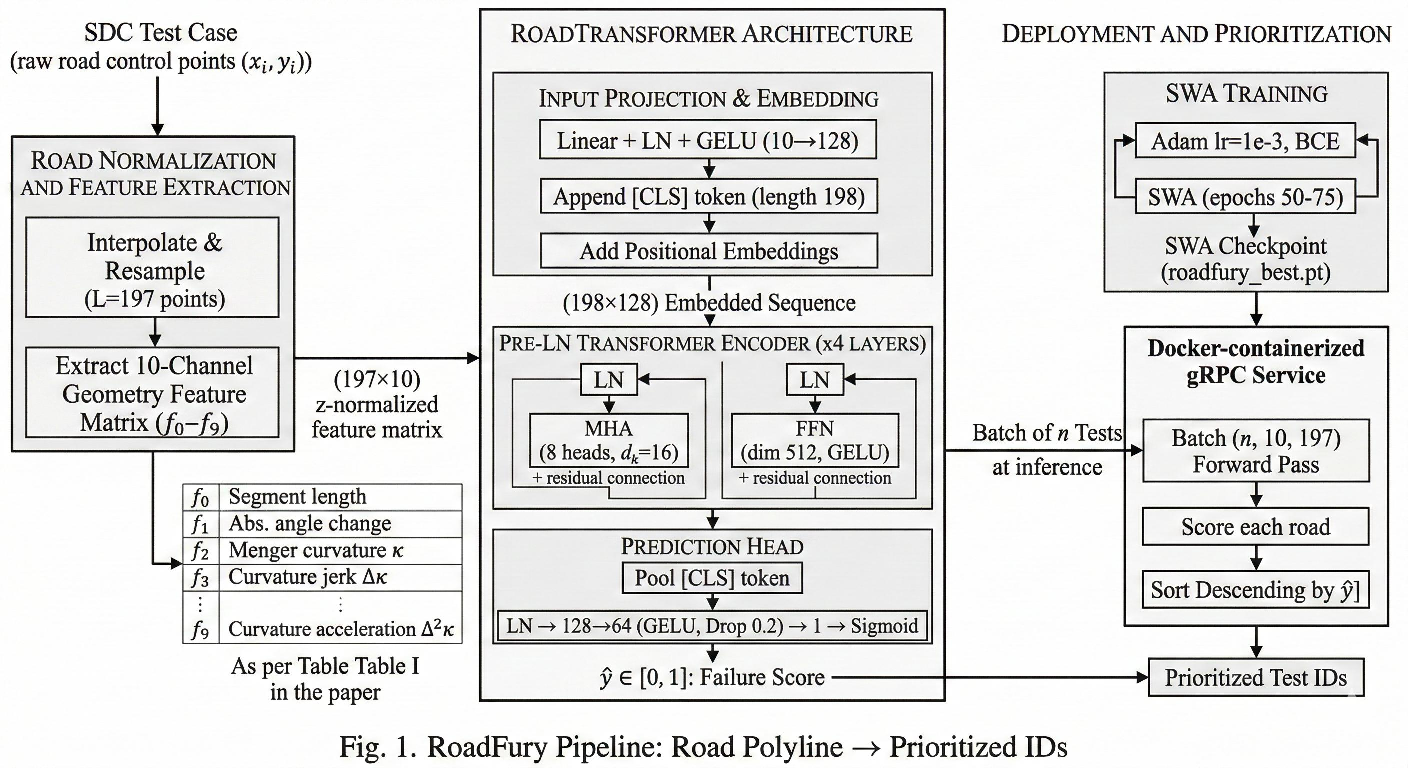
\includegraphics[width=\columnwidth]{fig1.pdf}
\vspace{-8pt}
\caption{RoadFury pipeline. Raw road control points are resampled, encoded into a 10-channel feature matrix, and processed by a Pre-LN Transformer Encoder. The \texttt{[CLS]} token summarizes the entire road; an MLP head converts it to a failure score $\hat{y}$ used for prioritization.}
\label{fig:arch}
\vspace{-4pt}
\end{figure}

\subsection{Training and Deployment}

We train with Adam (lr\,=\,$10^{-3}$) and binary cross-entropy for 75 epochs on the 28,804-sample training split. The key ingredient is \emph{Stochastic Weight Averaging} (SWA)~\cite{b6}: starting at epoch~50, the optimizer averages model weights over the remaining 25 epochs. This ensemble-in-weight-space finds a flatter region of the loss landscape, which is critical for generalization to unseen competition roads whose geometry distributions may differ from training.

At inference, the model scores all $n$ test cases in a single batched forward pass and returns them sorted by descending failure probability. The tool is packaged as a Docker-containerized gRPC service exposing three endpoints: \texttt{Name}, \texttt{Initialize} (receives labeled oracle data), and \texttt{Prioritize} (returns the ranked test order).

%=====================================================================
\section{Evaluation}

We evaluate on SensoDat~\cite{b7}, a corpus of 36,006 labeled BeamNG.tech simulation tests, split 80/20 for training (28,804) and validation (7,202). The 956-test competition set serves as the held-out evaluation target. All results are averaged over 30 stratified random trials.

\textbf{Why not just any ML model?} Before converging on a Transformer, we explored four fundamentally different paradigms (Table~\ref{tab:results}). Each represents a distinct hypothesis about how road geometry should be encoded.

\begin{table}[t]
\caption{Multi-Paradigm Comparison (956 comp.\ tests, 30 trials)}
\vspace{-2pt}
\begin{center}{\small
\setlength{\tabcolsep}{3pt}
\begin{tabular}{lcc}
\toprule
\textbf{Method} & \textbf{APFD} & \textbf{Paradigm} \\
\midrule
Random                   & 0.493              & -- \\
LLM zero-shot            & 0.487\,$\pm$\,0.019 & Qwen2.5-7B, 4-bit \\
GNN (road graph)         & 0.533\,$\pm$\,0.025 & 3-layer GCN+KNN \\
ResNet50 + XGBoost       & 0.572\,$\pm$\,0.013 & Road image CNN \\
CNN + Handcrafted        & 0.673\,$\pm$\,0.017 & ResNet50 + 44 feat. \\
ExtendedCNN-10ch         & 0.768\,$\pm$\,0.014 & 10-ch CNN, 28K data \\
ITEP4SDC                 & 0.781              & ONNX MLP, 3 feat. \\
\textbf{RoadFury (ours)} & \textbf{0.804\,$\pm$\,0.012} & \textbf{Transformer+SWA} \\
\bottomrule
\end{tabular}}
\label{tab:results}
\end{center}
\vspace{-2pt}
\end{table}

\emph{Language models fail at geometry.} We prompted Qwen2.5-7B~\cite{b16} in 4-bit quantization with a textual summary of each road's curvature statistics. It scored \emph{below} random-language models can discuss curves in the abstract but cannot reliably judge whether a specific curvature value is dangerous.

\emph{Graphs lose the sequence.} Representing road points as a graph with sequence and spatial KNN edges (3-layer GCN~\cite{b21}) captures local neighborhoods but discards the ordering that matters: a sharp turn preceded by a long straight is far more dangerous than the same turn after a gradual curve.

\emph{Images discard precision.} Rendering road polylines to $224{\times}224$ px images and extracting features via ImageNet-pretrained CNNs~\cite{b5} treats the road as a visual pattern. Even fused with 44 handcrafted features, this approach plateaus well below methods that preserve the raw numeric geometry.

\emph{Feature quality over model scale.} The most revealing comparison is between the ExtendedCNN-10ch and the pure CNN baselines: using our 10-channel features in a simple 1D-CNN already reaches 0.768, demonstrating that \emph{what} you measure matters more than \emph{how} you model it.

\emph{Attention captures what matters.} RoadFury's Transformer attends to all 197 road points simultaneously, learning which curvature transitions-not just which magnitudes-predict failures. Combined with SWA, this yields the highest APFD at 0.804\,$\pm$\,0.012.

\textbf{Ablation.} We tested seven modifications in isolation over the base Pre-LN Transformer. Multi-scale convolution stems, stochastic depth~\cite{b20}, alternative pooling, mixup~\cite{b19}, and test-time augmentation all \emph{degraded} performance. Focal loss~\cite{b18} offered a marginal gain. Only SWA~\cite{b6} consistently improved the result, confirming that the architecture is already well-matched to this task and that regularization in weight space, rather than architectural complexity, is the missing ingredient.

%=====================================================================
\section{Conclusion}

The central finding of this work is that \emph{how} road geometry is represented matters far more than model size or training tricks. Language models, graph networks, and visual CNNs each impose an inductive bias that discards the sequential curvature dynamics cars actually experience. A Pre-LN Transformer, operating directly on the ordered 10-channel geometric sequence, preserves this structure and achieves the best result (APFD\,=\,0.804\,$\pm$\,0.012), establishing a new state of the art for the ICST~2026 SDC Competition. Future work will explore online adaptation using labeled oracle data received at test time, and multi-scale SWA scheduling for even flatter optima. The tool is publicly available at \url{https://github.com/chisngyen/sdc-test-prioritization-novel}.

\begin{thebibliography}{00}
\bibitem{b1} C. Birchler, S. Khatiri, B. Bosshard, A. Gambi, and S. Panichella, ``Machine learning-based test selection for simulation-based testing of self-driving cars,'' \textit{EMSE}, vol.~28, no.~71, 2023.
\bibitem{b2} C. Birchler, N. Ganz, S. Khatiri, A. Gambi, and S. Panichella, ``Cost-effective simulation-based test selection with SDC-Scissor,'' in \textit{Proc. IEEE SANER}, 2022, pp.~386--390.
\bibitem{b4} S. Yoo and M. Harman, ``Regression testing minimization, selection and prioritization: A survey,'' \textit{STVR}, vol.~22, no.~2, pp.~67--120, 2012.
\bibitem{b5} A. Vaswani et al., ``Attention is all you need,'' in \textit{NeurIPS}, vol.~30, 2017.
\bibitem{b6} P. Izmailov, D. Podoprikhin, T. Garipov, D. Vetrov, and A. G. Wilson, ``Averaging weights leads to wider optima and better generalization,'' in \textit{Proc. UAI}, 2018.
\bibitem{b7} C. Birchler, S. Khatiri, and S. Panichella, ``SensoDat: Simulation-based sensor dataset of self-driving cars,'' 2024.
\bibitem{b8} P. Aryan, T. Fulcini, L. Starace, C. Birchler, and S. Panichella, ``{ICST} Tool Competition 2026 - SDC Testing Track,'' in \textit{Proc. IEEE ICST}, 2026.
\bibitem{b11} R. Xiong et al., ``On layer normalization in the Transformer architecture,'' in \textit{Proc. ICML}, 2020.
\bibitem{b14} D. S. Duy Minh, T. K. Huynh, et al., ``Early-stage prediction of review effort in AI-generated pull requests,'' in \textit{Proc. IEEE/ACM MSR}, 2026.
\bibitem{b15} T. K. Huynh, D. S. Duy Minh, et al., ``Systematic evaluation of ML and Transformer methods for scientific literature classification,'' in \textit{Proc. TRACS@WASP}, 2025.
\bibitem{b16} P. H. Pham, C. N. Tran, D. S. Duy Minh, et al., ``Navigating simply, aligning deeply: Winning solution for Mouse vs.\ AI 2025,'' in \textit{NeurIPS 2025 Competition Track}, 2026.
\bibitem{b17} L. P. Q. Nguyen, D. S. Duy Minh, et al., ``Beyond vision: Contextually enriched image captioning,'' in \textit{ACM MM EVENTA}, 2025. arXiv:2512.20042.
\bibitem{b18} T.-Y. Lin, P. Goyal, R. Girshick, K. He, and P. Doll\'ar, ``Focal loss for dense object detection,'' in \textit{Proc. ICCV}, 2017.
\bibitem{b19} H. Zhang, M. Ciss\'{e}, Y. N. Dauphin, and D. Lopez-Paz, ``Mixup: Beyond empirical risk minimization,'' in \textit{Proc. ICLR}, 2018.
\bibitem{b20} G. Huang, Y. Sun, Z. Liu, D. Sedra, and K. Q. Weinberger, ``Deep networks with stochastic depth,'' in \textit{Proc. ECCV}, 2016.
\bibitem{b21} T. N. Kipf and M. Welling, ``Semi-supervised classification with graph convolutional networks,'' in \textit{Proc. ICLR}, 2017.
\end{thebibliography}

\end{document}
